% This file demonstrates the use of the `WindForS` style
% ---------------
% PREAMBLE
% ---------------
\documentclass[twocolumn,a4paper]{article}

\usepackage[blackLinks=false, logo = true]{WindForS}

% -----------------------------------
% DOCUMENT PROPERTIES
% -----------------------------------
\title{Writing WindForS Articles using LaTeX}
\shorttitle{LaTeX for WindForS}
\author{A. Clifton}
\addbibresource{../common_files/bibliography.bib}
\setcounter{tocdepth}{1}
% need to remove
% -------------------------------------
% DOCUMENT STARTS HERE
% -------------------------------------
\begin{document}
\maketitle

\section*{Executive Summary}
This document is a guide to writing corporate documents using the LaTeX document preparation system.

LaTeX is not WYSIWYG and has different reviewing and editing tools compared to typical word processing software. For this reason special care has to be taken when preparing documents in LaTeX. 

This document also serves as a template. It is intended for people with some familiarity with LaTeX.
\tableofcontents
\listoffigures
\listoftables

\lstset{language=[LaTeX]Tex, columns=fullflexible, keepspaces=true,breaklines=true}
%% CHAPTER: WHAT IS LATEX
\chapter{What is LaTeX?}
LaTeX is a mark-up language that describes how a document should be prepared.

Three things are needed to make a LaTeX document:
\begin{enumerate}
\item A source document, usually with extension \emph{.tex}
\item Some packages and classes that help turn what's in the source document into something helpful
\item A compiler, also referred to as a working LaTeX installation. This could be local or web-based, for example at \href{www.overleaf.com}{overleaf.com}.
\end{enumerate}

At first glance the source document looks like a programming language, and that's because it is: LaTeX is not WYSIWYG, like many of the document preparation tools in common use today. A good analogy to LaTeX is html code, which can be read in any text editor but is rendered by web browsers into a finished product.


\section{Printed Resources}
Several excellent LaTeX references exist and may be found useful by some users. Examples include those by \citet{Knuth_1984_a} and \citet{Lamport_1986_a}.


\section{Online Resources}
Several excellent LaTeX references exist and may be found useful by some users. Examples include those by \citet{Knuth_1984_a} and \citet{Lamport_1986_a}.

%% CHAPTER: HOW TO MAKE LATEX DOCUMENTS %%
\section{Using LaTeX to Make Corporate Documents }
A series of LaTeX class files called \emph{Corporate...cls} have been written to implement common formatting requirements in LaTeX.

\subsection{WindForS style files}\label{sec:Corporatecls}
Style files control the formatting and presentation of \LaTeX documents. These are available as \emph{packages} for different journals, institutions, and other applications. 

A WindForS style file has been written to format documents created with the latex \texttt{article}, \texttt{scrartcl}, and \texttt{book} classes. The usual options can still be used with the document classes, including \emph{twocolumn, letterpaper}, and so-on.

Options can be passed to the WindForS style in the preamble:

\begin{lstlisting}
\usepackage[option 1 = true, ..., option n= string]{WindForS}
\end{lstlisting}

Options include:
\begin{description}
\item[blackLinks = true]{make all links the same color as the rest of the body text.}
\item[compactLayout = true]{reduce white space around headings and lists.}
\item[draft = true]{add a `draft' watermark to all pages.}
\item[logo = true]{show the WindForS logo in headers (defaults to true).}
\item[logoPath = ...]{use a specific file for the logo (defaults to \emph{./logo.png}).}
\item[coverLogoPath = ...]{use a specific file for the logo on the front cover of reports (defaults to \emph{./logo\_windfors\_uz\_d\_e.png}).}
\end{description}

The \emph{WindForS} package calls other packages listed in Table \ref{tab:incpacks}. These packages often call other packages, so this is not an exhaustive list.

\begin{table}[!ht]
\centering
\caption[Packages loaded by the corporate style]{Packages loaded by the corporate style.}
\label{tab:incpacks}
\begin{tabular}{p{0.3\columnwidth}p{0.6\columnwidth}}
\toprule
Package &  Functionality\\
\midrule
%accessibility & tagged & generates the document structure and tagging \\
amsfonts, amssymb & supplies AMS fonts, which are useful for mathematics \\
babel &  activates language-appropriate hyphenation rules\\
booktabs & improves the formatting of tables \\
caption & required to generate captions for floats\\
courier& changes fonts \\
fontenc &  enables direct typing of international characters \\
geometry & sets page size and margins \\
graphicx & graphics handling, including \emph{.eps} figures \\
hyphenat & improves spacing and breaking of hyphenated words \\
listings & enables the inclusion of high-quality computer code listings\\
mathptmx& changes fonts \\
nag & checks that packages are up to date and looks for bad habits in LaTeX code\\
opensans& sets Google's \emph{Open Sans} as the default font\\
parskip & required for better spacing\\
pdfcomment & required for tool-tips. Also calls the \texttt{hyperref} package.\\
setspace & required for better spacing\\
subcaption & provides the \texttt{subfigure} environment to produce sub figures \\
tocloft & improved table of contents and list of figures/tables in memoir documents\\
tocbibind &  Adds bibliography, index, and contents entries to the Table of Contents in memoir documents\\
todonotes &  inline and margin to-do notes \\
xcolor &  Driver-independent color extensions for LaTeX and pdfLaTeX\\
\bottomrule
\end{tabular}
\end{table}

It should be noted that the `english` option to Babel really means American English.

\subsection{Starting new documents}\label{sec:NewDocs}
\begin{enumerate}
\item Go to \href{https://github.com/xx}{https://github.com/xx} and download the latest version of the repository as a .zip file from the icon on the lower right hand side of the page.
\item Modify \emph{main*.tex} as required.
\end{enumerate}


\subsection{Creating content}
\subsubsection{Front, main, and back matter}
The convention in this corporate class is to have Roman numerals in the front matter, and then arabic numerals in the main matter of the document (after the tables of contents, figures and tables). Tables and figures in the front matter are also numbered differently (Table A, B, C, ...) than in the main matter (Table 1, 2, 3, ...).

This change in page and float numbering is implemented using the \verb+\frontmatter+, \verb+\mainmatter+, and \verb+\backmatter+ commands at the start of these sections of the document:

\begin{lstlisting}
\begin{document}

\maketitle
\frontmatter
...
\tableofcontents
\clearpage
\listoffigures
\listoftables
\mainmatter
...
\backmatter
\end{document}
\end{lstlisting}

Page numbering in the front matter (i.e. the Abstract, Summary, and Foreword chapters or sections) starts at page 3 to allow for cover pages.

If you don't use the \verb+\frontmatter+ commands, you may need to increment the page counter manually. To increment the counter $n$ pages, use \verb+\setcounter{page}{n}+ after \verb+\begin{document}+.

\subsubsection{Cross references}
Use labels and references to refer back and forth to figures, equations, tables and sections. 

For example, an equation can be added using the following text:

\begin{lstlisting}
\begin{equation}
y = mx+c
\label{eqn:line}
\end{equation}
\end{lstlisting}

This gives the following:
\begin{equation}
y = mx+c
\label{eqn:line}
\end{equation}

And using the text \verb+Eqn. \ref{eqn:line}+ provides a cross reference to Eqn. \ref{eqn:line}.

\subsubsection{Floats}
Floats are images, tables or other pieces of the document that are free to move to the best place in the document for them. The two most common floats are the tabular environment (for tables) and the figure environment for figures.

Use the \texttt{tabular} environment to produce basic tables. Table~\ref{tab:widgets} is produced using this code: 

\begin{lstlisting}
\begin{table}[!h]
\centering
\caption{An example table.}\label{tab:widgets}
\begin{tabular}{lr}
Item & Quantity \\
\hline
Widgets & 42 \\
Gadgets & 13
\end{tabular}
\end{table}
\end{lstlisting}

\begin{table}[!h]
\centering
\caption{An example table.}\label{tab:widgets}
\begin{tabular}{lr}
Item & Quantity \\
\hline
Widgets & 42 \\
Gadgets & 13
\end{tabular}
\end{table}

If all of the delimiters (\&) are included in each row, the table will be complete and will produce a better PDF.

To include a figure in a document, use the \texttt{figure} environment and the \texttt{includegraphics} command.

\begin{lstlisting}
\begin{figure}
\includegraphics[width=\textwidth]{figure's-file-name}
\caption{Caption goes here.}\label{fig:figuresLabel}
\end{figure}
\end{lstlisting}

Subfigures are implemented using the \texttt{subcaption} package. The example below generates Figure \ref{fig:NRELimages}.

\begin{lstlisting}
\begin{figure*}
	\centering
        \begin{subfigure}[t]{.45\linewidth}
		\centering
		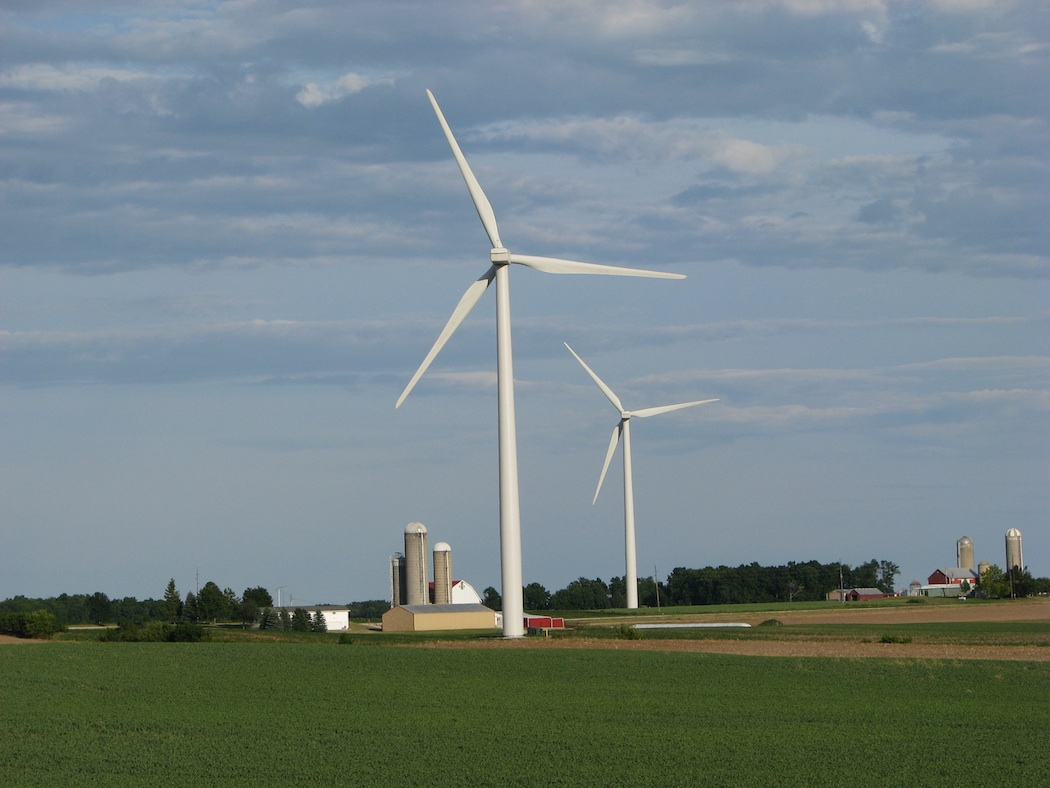
\includegraphics[height=2in]{../DemoFiles/21206}
		\caption{Wind turbines at the Forward Wind Energy Center in Fond du Lac and Dodge Counties, Wisconsin. (Photo by Ruth Baranowski / NREL)}\label{fig:21206}
	\end{subfigure}%
        \hfill
        \begin{subfigure}[t]{.45\linewidth}
		\centering
		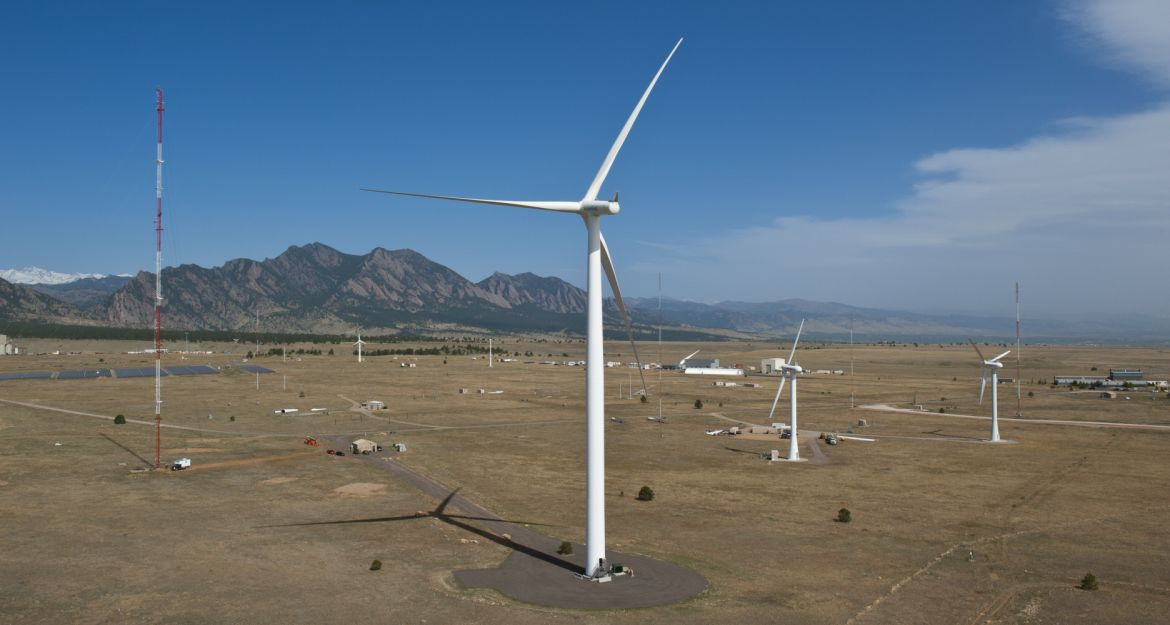
\includegraphics[height=2in]{../DemoFiles/20018}
		\caption{Aerial view of the National Wind Technology Center. (Photo by Dennis Schroeder / NREL)}\label{fig:20018}
	\end{subfigure}
	\caption{Images}\label{fig:NRELimages}
\end{figure*}
\end{lstlisting}

Note that the \texttt{subfig} and \texttt{subfigure} packages are deprecated. The \texttt{subcaption} package appears to be the most frequently maintained package at this time, and contains the same functionality as the \texttt{subfig} and \texttt{subfigure} packages.

\begin{figure*}
	\centering
        \begin{subfigure}[t]{.45\linewidth}
		\centering
		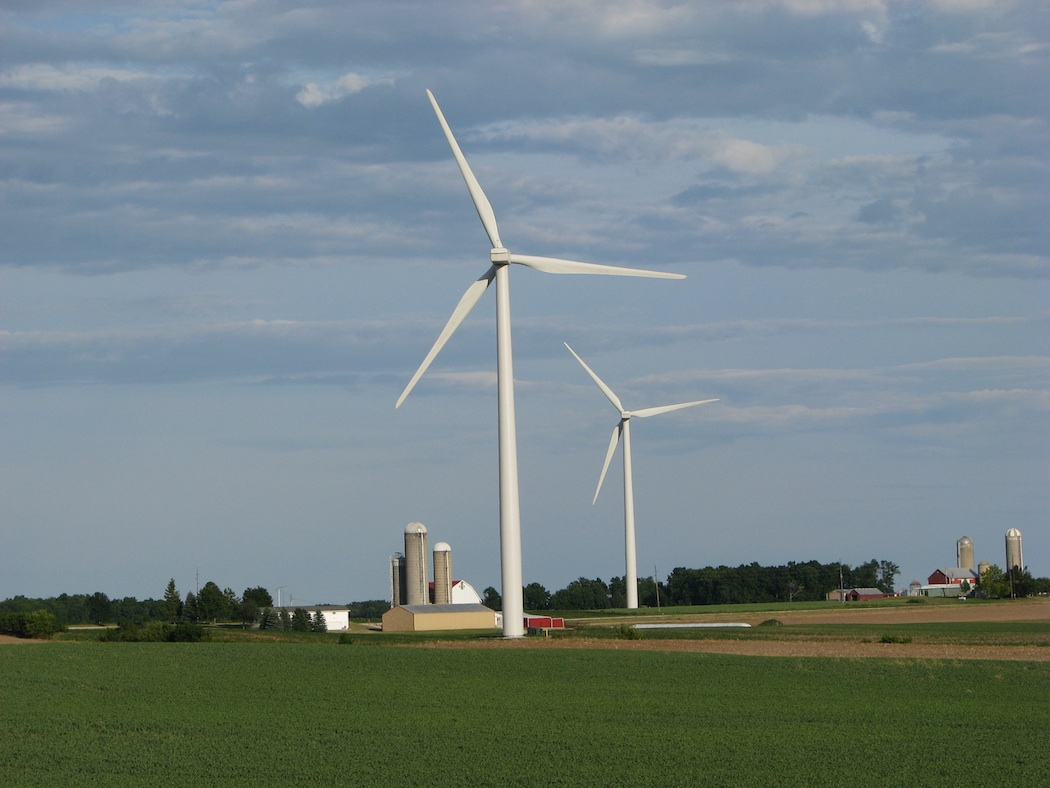
\includegraphics[height=2in]{../DemoFiles/21206}
		\caption{Wind turbines at the Forward Wind Energy Center in Fond du Lac and Dodge Counties, Wisconsin. (Photo by Ruth Baranowski / NREL)}\label{fig:21206}
	\end{subfigure}%
        \hfill
        \begin{subfigure}[t]{.45\linewidth}
		\centering
		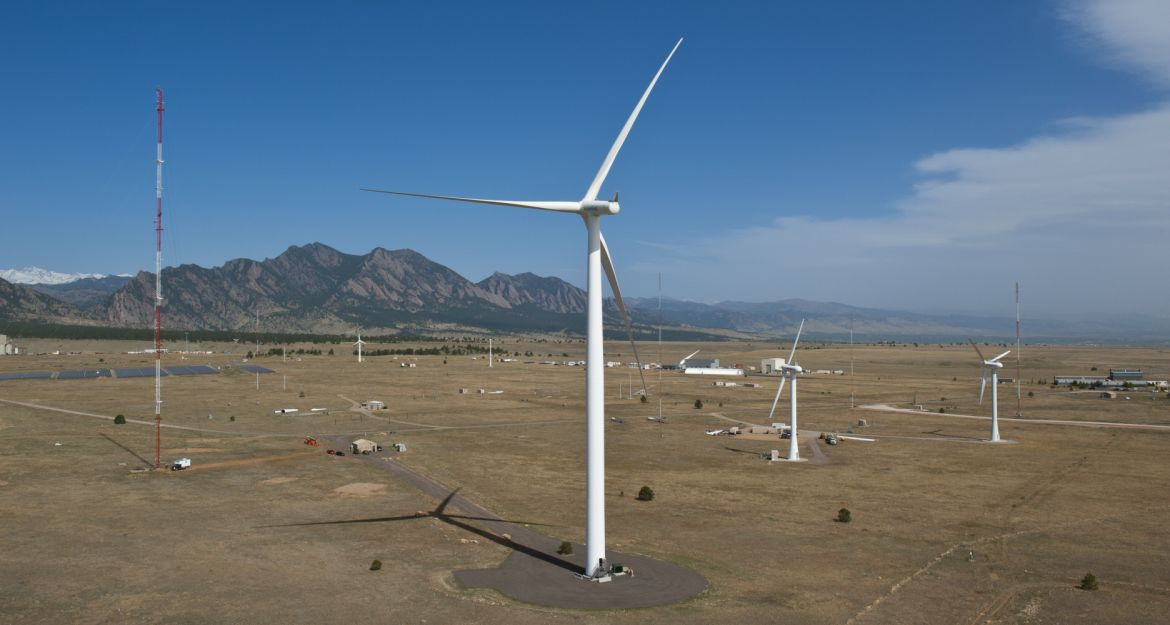
\includegraphics[height=2in]{../DemoFiles/20018}
		\caption{Aerial view of the National Wind Technology Center. (Photo by Dennis Schroeder / NREL)}\label{fig:20018}
	\end{subfigure}
	\caption{Images}\label{fig:NRELimages}
\end{figure*}


\subsubsection{Including computer code}\label{Sec:Codes}
The \texttt{listings} package has been loaded. Note: this does not work if the `Draft' document option is used.

To insert code with syntax highlighting, you can use the \texttt{lstlisting} environment, for example \verb+\begin{lstlisting} ...\end{lstlisting}+.

You can change the language that is used to control the syntax highlighting using \verb+\lstset{language=[dialect]language}+. For example, this document uses...

\begin{lstlisting}
\lstset{language=[LaTeX]Tex,columns=fullflexible,keepspaces=true,breaklines=true}
\end{lstlisting}

... because most of the code is LaTeX. This can be changed for each block of code, however (and should be changed back afterwards). For example, the next block of code is written in C.

\lstset{language=c}
\begin{lstlisting}

/* Hello world in C* */

#include <stdio.h>

main()
{
    printf("Hello World!\n");
}
\end{lstlisting}

\lstset{language=[LaTeX]Tex}

For more details see the \texttt{lstlisting} documentation or the \href{https://en.wikibooks.org/wiki/LaTeX/Source_Code_Listings}{wikibook}.

\subsubsection{Citations}\label{Sec:Citations}
Use \texttt{bibtex} to organize references and store them in a single file (e.g. \verb+/Documents/bibliography/bibliography.bib+). The bibliography will then contain entries with `keys' for each source, like \texttt{Lamport\_1986\_a}. 

Authors can then insert citations to this key throughout their document, using different styles of citation. Citations are generated using the \texttt{biblatex} package, which also formats references in the correct style.  Ways to generate citations are described in the \texttt{biblatex} documentation, and include:
\begin{itemize}
\item \verb+\cite{Lamport_1986_a}+ prints \cite{Lamport_1986_a}.
\item \verb+\citep{Lamport_1986_a}+ prints \citep{Lamport_1986_a}.
\item \verb+\citet{Lamport_1986_a}+ prints \citet{Lamport_1986_a}.
\end{itemize}

To cite URLs, use the 'misc' style. For example, the bibtex entry for \href{http://tex.stackexchange.com}{http://tex.stackexchange.com}\ \citep{texstackexchange} looks like this:

\begin{lstlisting}
@misc{texstackexchange,
	Author = {Anon.},
	Howpublished = {Accessed July 21, 2014: \url{http://tex.stackexchange.com}},
	Title = {\TeX -- LaTeX Stack Exchange},
	Year = {2014}}
\end{lstlisting}

This format will allow you to include the date on which a URL was accessed.

The citations should work with journal articles \citep{Clifton_2013_a}, books \citep{Knuth_1984_a, Lamport_1986_a, chicago}, technical reports \citep{TechReportTest}, and URLs \citep{texstackexchange}. Any unknown publication types will be formatted using the `misc' type.


\subsubsection{Bibliographies}\label{Sec:Bibliographies}
This document class uses "Chicago A" style-references produced using Biblatex. The reference style can be changed in the \emph{CorporateArticle.cls} file.

To include a bibliography in the document give the bibliography file location in the preamble and insert the bibliography at the appropriate location:

\begin{lstlisting}
% give the bibliography file location
\bibliography{files/bibliography.bib}
...
\begin{document}
...
% insert the bibliography into the document
\cleardoublepage
\label{sec:Bib}
\printbibliography
...
\end{document}
\end{lstlisting}

An example bibliography is included in this document on page \pageref{sec:TheBibliography}.

\subsubsection{Footnotes}
Footnotes can be inserted using the \verb+\footnote{}+ command\footnote{like this}. Footnotes are numbered in the main matter\footnote{and like this as well}, and use daggers, etc instead of numers in the appendices.


\subsection{Creating a file structure}\label{sec:FileStructure}
Your main file should be called \emph{main.tex}. This helps editors and coauthors identify where to start. Then, use \texttt{input} to import other files into your main file at compilation.

For example, each of the chapters in this report is in separate files, called \emph{WhatIsLatex} (Chapter 1), \emph{LatexForDocs} (Chapter 2), and so-on. In the example available on Github, they are stored in the \emph{files} directory. \emph{main.tex} then looks like this:

\begin{lstlisting}
...
\begin{document}
% content
\chapter{What is LaTeX?}
\input{../common_files/WhatIsLaTeX_Intro.tex}

\section{Printed Resources}
\input{../common_files/WhatIsLaTeX_PrintResources.tex}

\section{Online Resources}
\input{../common_files/WhatIsLaTeX_PrintResources.tex}
\input{files/LatexForDocs}
...
\end{lstlisting}


\subsection{Best practice in writing a document in LaTeX}
\begin{description}
\item[Create a structure before you get too far.] Authors will find it easier to write documents and make changes if they separate the content of the document from the structure.
\begin{enumerate}
\item Each new LaTeX document should be placed in it's own directory. 
\item Create a main LaTeX file that just contains the preamble, custom commands and uses \texttt{input} to call the content. See Section \ref{sec:FileStructure} for an example where each \texttt{chapter} is contained in its own file. In an article, each \texttt{section} could be contained in its own file.
\item Keep the number of packages used to a minimum. Not all packages can be used as they lack compatibility.
\end{enumerate}
\item[Focus on content, not appearance.] Don't spend hours trying to adjust fonts, headers or spacing between lines. 
\begin{enumerate}
\item Don't throw in lots of \texttt{clearpage}s or other commands to push material around. LaTeX is designed to handle that. 
\item Resist the temptation to add or subtract space, change lengths or do other things to modify the layout. 
\item Write!
\end{enumerate}
\end{description}

%% CHAPTER: MAKING PDFS
\section{Preparing an Accessible PDF from LaTeX}\label{sec:PDFPrep}
Care has to be taken to produce a PDF that meets best practice for accessibility. This may require special steps such as tagging, alt-text, and embedding fonts for documents that will be used with electronic document readers.

\subsection{PDF tagging}\label{sec:PDFPrep_Tagging}
PDF tagging is a process whereby the components of the PDF document (headings, figures, tables, text) are marked so that a document reader can understand the document. This is useful when text to speech converters are being used. The process of tagging is also known as structuring, so that a tagged document might also be referred to as a structured document\footnote{This is a test}.

\LaTeX\ does not prepare a structured PDF document directly.

At this time tags cannot be added reliably within LaTeX. Instead, they should be added after the PDF is compiled using a PDF editor such as Adobe's Acrobat Pro. 


\subsection{Alternative text}\label{sec:PDFPrep_AltText}
Alternative text, or `Alt text', is a textual description of an equation, link or figure that can be used to replace the visual information in that element. This is often seen as a text `pop-up' in PDF readers. 

At this time Alt text cannot be added reliably withing LaTeX. Instead, it should be added after the PDF is compiled using a PDF editor such as Adobe's Acrobat Pro. 


\subsection{Embedded fonts}\label{sec:PDFPrep_EmbeddedFonts}
All fonts should be embedded in the the final PDF. Check the PDF for embedded fonts using a PDF viewer. For example, in Adobe Acrobat Reader, look at the `fonts' tag of the document properties. If any fonts are not shown as being an \emph{embedded subset}, try the conversion again. 

Encapsulated postscript figures are particularly prone to having undefined fonts. Check by compiling the document in draft mode, and seeing if the fonts are still present in the output PDF. To fix this problem, change \emph{.eps} files to \emph{.png} files. To do this `on the fly', use this in the document's preamble:

\begin{lstlisting}
\usepackage{epstopdf}
\epstopdfDeclareGraphicsRule
 {.eps}{png}{.png}{convert eps:\SourceFile.\SourceExt png:\OutputFile}
\AppendGraphicsExtensions{.png}
\end{lstlisting}
%% ACK
\section*{Acknowledgments}
This document is based on the NREL LaTeX class files developed by the author and then forked for this project.

I wish to thank members of the TeX -- LaTeX StackExchange site for useful suggestions concerning LaTeX and typography \citep{texstackexchange}.

This report was typeset using the LaTeX typesetting system originally developed by Leslie Lamport, based on TeX created by Donald Knuth.
%% CHAPTER: APPENDICES

% bibliography
\label{sec:TheBibliography}
\printbibliography

\appendix
\section{How to Use Appendices}
Appendices can be included in \emph{Corporate*.cls} documents. 


\subsection{How to switch to appendixes}
To switch to appendices, use the \emph{appendix} command:

\begin{lstlisting}
\appendix
\section{How to Use Appendices}
\input{../DemoFiles/AppendixA_Intro}

\subsection{How to switch to appendixes}
\input{../DemoFiles/AppendixA_Switch}

\subsection{Changes to Figure, Table, and Footnote Numbering}
\input{../DemoFiles/AppendixA_Numbering}
\section{Including Multiple Appendices}
\input{../DemoFiles/AppendixB_Intro}

\subsection{Changes to numbering}
\input{../DemoFiles/AppendixB_Numbering}

\end{lstlisting}

\subsection{Changes to Figure, Table, and Footnote Numbering}
The following table (Table \ref{tab:AppAWidgets}) should have a different caption numbering style than Table \ref{tab:widgets}. The table number should start with the appendix label (in this case \thesection,) be followed by a period, and then be numbered. Numbering should restart in each new appendix.

\begin{table}[!ht]
\centering
\caption{An example table.}\label{tab:AppAWidgets}
\begin{tabular}{lr}
Item & Quantity \\
\hline
Widgets & 42 \\
Gadgets & 13
\end{tabular}
\end{table}

The following table should use the same letter as Table \ref{tab:AppAWidgets}, but the number should be incremented by one.

\begin{table}[!ht]
\centering
\caption{An example table.}\label{tab:AppAWidgetsTwo}
\begin{tabular}{lr}
Item & Quantity \\
\hline
Widgets & 42 \\
Gadgets & 13
\end{tabular}
\end{table}

Footnotes use symbols in place of numbers in the appendices\footnote{this is a test}.
\section{Including Multiple Appendices}
This chapter is included to demonstrate that the \emph{Corporate*.cls} file correctly formats a second appendix\footnote{this is also a test}.

\subsection{Changes to numbering}
The following table (Table \ref{tab:AppBWidgets}) caption should have a different numbering style than Table \ref{tab:widgets}. Instead, the caption numbering style should be the same as Table \ref{tab:AppAWidgets}. Numbering in this chapter should start with \thesection.

\begin{table}[!h]
\centering
\caption{An example table.}\label{tab:AppBWidgets}
\begin{tabular}{lr}
Item & Quantity \\
\hline
Widgets & 42 \\
Gadgets & 13
\end{tabular}
\end{table}



\end{document}
